\chapter{\IfLanguageName{dutch}{Evaluatieproces}{Evaluationproces}}%
\label{ch:evaluatieproces}
\section{Inleiding}
Het interpreteren van gevoelens en boodschappen uit kunstwerken is een zeer persoonlijk iets. Het beoordelen van de effectiviteit van de applicatie is dus een uitdagende taak zijn. Om een grondige evaluatie van onze kunstwerken mogelijk te maken, is er besloten om een Turingtest te implementeren als onderdeel van ons evaluatieproces. Hierbij werken we met een diverse set persona's. \\

Het doel van ons evaluatieproces is om de interpretatie en relevantie van de kunstwerken te valideren. Het resultaat van de turingtest kun je vinden in punt \ref{section:result}.

\section{Turingtest}
\label{sec:turingtest}
 Door deelnemers te vragen specifiek nieuws te identificeren dat zij associëren met elk schilderij, kunnen we hun begrip van de context en hun vermogen om de artistieke interpretatie te verbinden met actuele gebeurtenissen beoordelen. We zullen de deelnemers vragen om specifieke nieuwsgebeurtenissen te identificeren die zij associëren met elk schilderij.  Indien een deelnemer een onjuiste associatie maakt, zullen we het betreffende nieuwsartikel tonen en vervolgens vragen of ze het nieuwsgebeuren herkennen.. Indien een deelnemer geen nieuws volgt, kunnen we hem altijd vragen te gokken naar wat er zou kunnen ge-associeerd zijn met deze kunstwerk om te weten welk gevoel of boodschap dit overbrengt. \\
 
 In deze test zullen we deelnemers vragen om drie verschillende schilderijen te bekijken, elk verkregen door de de applicatie van de laatste drie dagen. De taak van de deelnemers is om aan te geven welk nieuwsgebeuren zij herkennen in elk van de schilderijen. Het resultaat van deze 3 samples laat ons toe om te kunnen oordelen of de applicatie goed zou kunnen werken binnen bijvoorbeeld een krant of nieuwswebsite.  \\
 
 Verder voegen we ook 2 samples toe die zeer belangrijke data zijn uit het verleden, we zullen hiervoor de scraper moeten aanpassen zodat deze op een specifieke dag kan scrapen. Het resultaat van deze 2 samples laat ons toe om te kunnen oordelen of AI wel degelijk in staat is om schilderijen te genereren waarvan de boodschap de kernboodschap is van de dag. De wijzigingen aan de code vind je in bijlage \ref{bijlage:changes_scraper}
 

  
\section{Persona}

Zoals eerder vermeld hebben we tijdens de turingtest een diverse groep deelnemers betrokken. We hebben verschillende criteria gehanteerd, zoals leeftijd, geslacht, artistieke achtergrond, huidige baan of studie, en of de persona het nieuws volgt of niet. \\

Naast deze diversiteit in persoonlijke kenmerken hebben is er ook voor gekozen om persona's uit verschillende landen te betrekken, namelijk Nederland en Litouwen. We hebben hiervoor gekozen omdat perspectieven en percepties vaak verbonden zijn aan cultuur en achtergrond. Door de betrokkenheid van verschillende nationaliteiten kunnen we de invloed van deze diverse perspectieven op de interpretatie van kunstwerken onderzoeken.

\begin{table}[htbp]
    \centering
    \begin{tabular}{|p{2cm}|p{1.3cm}|p{1.4cm}|p{2.8cm}|p{4cm}|p{1.5cm}|}
        \hline
        Voornaam & Leeftijd & Geslacht & Artistieke Achtergrond  & Job of studies & Volgt het nieuws \\
        \hline
        Ronan & 24 jr. & Man & Tekenen &  ICT  & Neen  \\
        
        Arthur & 20 jr. & Man & Geen & ICT & Neen \\ 
        
        Arjan & 37 jr. & Man & Graphic Design & Projectmanager & Soms \\
        
        Lucas & 24 jr. & Man & Muziek & Software Engineer & Neen \\
        
        Gustas & 23 jr. & Man & Kunstschool & Eigen baas & Neen \\ 
        
        Shauny & 23 jr. & Vrouw & Geen & Journalistiek & Ja \\
 
        Filip & 56 jr. & Man & Schilderen & Buschauffeur &  Ja \\

        Marta & 47 jr. & Vrouw & Geen & Leerkracht & Ja \\
        \hline

    \end{tabular}
    \caption{Informatie over de persona's}
    \label{table:persona}
\end{table}

\section{Samples}
Alle persona's, beschreven in de vorige tabel \ref{table:persona}, worden bevraagd aan de hand van 3 schilderijen. Deze schilderijen representeren de belangrijkste nieuwsgebeurtenissen van dit weekend, waarbij één artikel een boodschap overbrengt die dateert van maandag. Aangezien de test op dinsdag plaatsvindt, zal er maximaal 3 dagen tussen het oudste schilderij zitten. \\

In de tabel hieronder vindt u de 3 schilderijen, inclusief de datum en de gebruikte prompt. Nadat we de prompt hebben ontvangen, stellen we de vraag aan GPT: 'Op basis van welke kernartikelen heb je dit gegenereerd?'. Het antwoord hierop wordt ook weergegeven in de tabel terug te vinden in tabel \ref{table:samples}
Daarnaast zijn er ook 2 extra samples toegevoegd die bekende gebeurtenissen uit het verleden representeren zoals vermeld in punt \ref{sec:turingtest}. Deze tabel is terug te vinden in punt \ref{table:events_samples}

    \begin{table}[htbp]
        \centering
        \begin{tabular}{|p{2cm}|p{4.7cm}|p{4.7cm}|p{4.7cm}|}
            \hline
            & 
            \adjustbox{width=4cm,padding=5pt}{
\includegraphics{./graphics/sample_1.png}} &
            \adjustbox{width=4cm,padding=5pt}{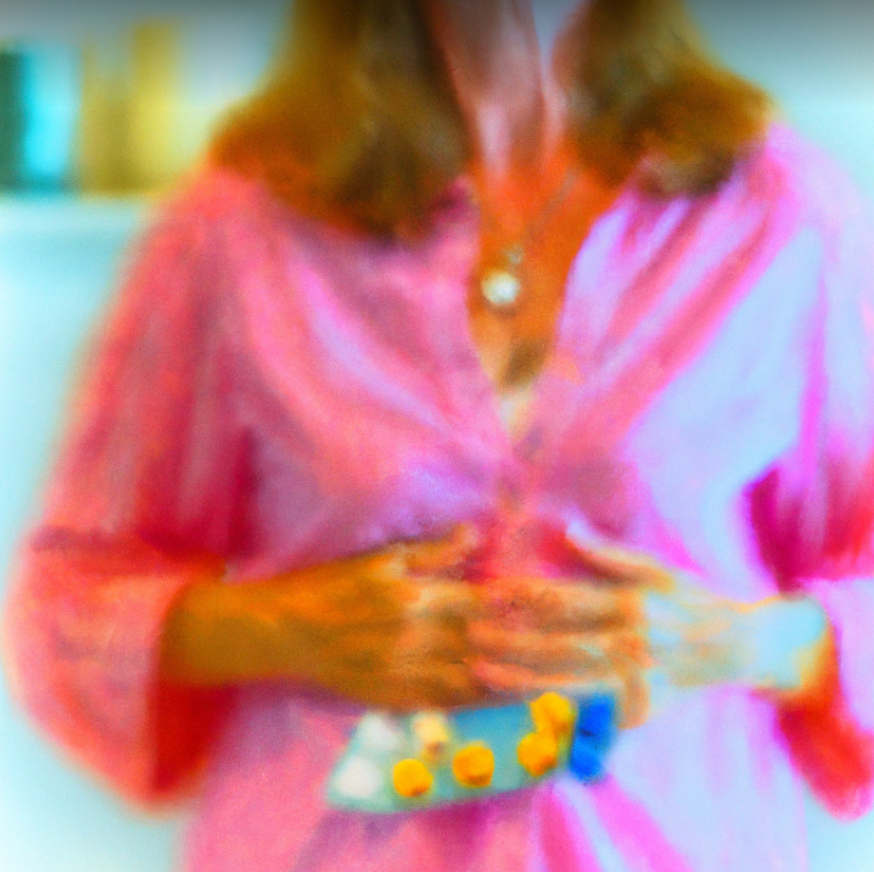
\includegraphics{./graphics/sample_2.png}} &
            \adjustbox{width=4cm,padding=5pt}{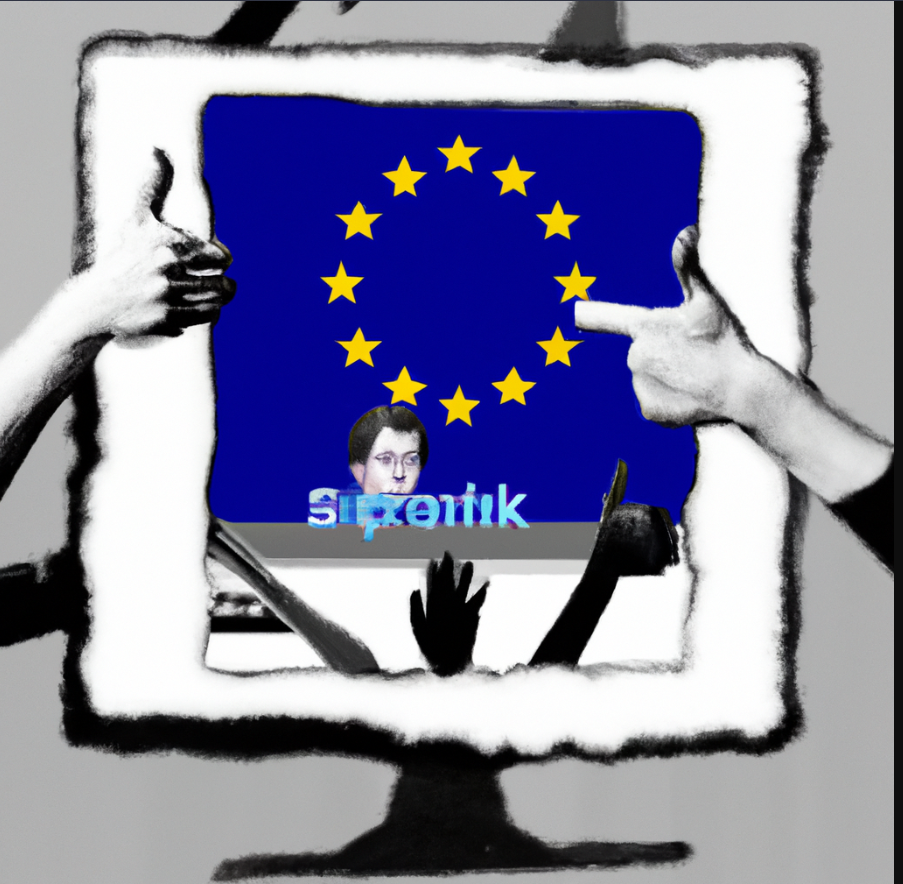
\includegraphics{./graphics/sample_3.png}} \\
            \hline
            \textbf{Referentie} & \textbf{Sample 1} & \textbf{Sample 2} & \textbf{Sample 3} \\
            \hline
            Datum & Zaterdag 20 Mei & Zondag 21 Mei & Maandag 22 Mei \\
            \hline
            Gebruikte prompt & "Eenheid voor Oekraïne" in Realistische stijl. &Women's Menopause Symptoms Relieved by Promising New Drug Style: Impressionism. & "Europese Unie geeft Facebook's Meta een recordboete" - Stijl: Surrealisme . \\
            \hline
            Inspiratie  (volgens GPT) & De prompt was gebaseerd op de kernboodschap die  eerder had gegenereerd op basis van het artikel over Charles Michel en de G7-landen die een langetermijnhulpplan en druk uitoefenden voor Oekraïne. & De kernboodschap die ik heb gegenereerd, is gebaseerd op het artikel "Nieuw medicijn tegen opvliegers op komst: ‘60 tot 70 procent van de vrouwen heeft er last van’", dat in het gegeven JSON-bestand wordt genoemd. & Deze prompt is afgeleid van de belangrijkste titel uit de JSON-gegevens die door de gebruiker zijn verstrekt, met name: "EU geeft Facebook-moederbedrijf Meta recordboete van 1,2 miljard euro". Ik heb de titel verkort tot een gepaste lengte. \\
            \hline
        \end{tabular}
        \caption{Eerste 3 gebruikte samples binnen de turingtest.}
        \label{table:samples}
    \end{table}


    \begin{table}[htbp]
    \centering
    \begin{tabular}{|p{2cm}|p{5.3cm}|p{5.3cm}|}
        \hline
        & 
        \adjustbox{width=5cm,padding=5pt}{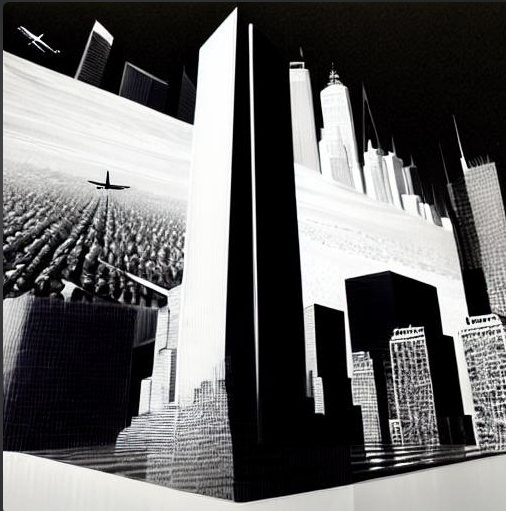
\includegraphics{./graphics/sample_4.png}} &
        \adjustbox{width=5cm,padding=5pt}{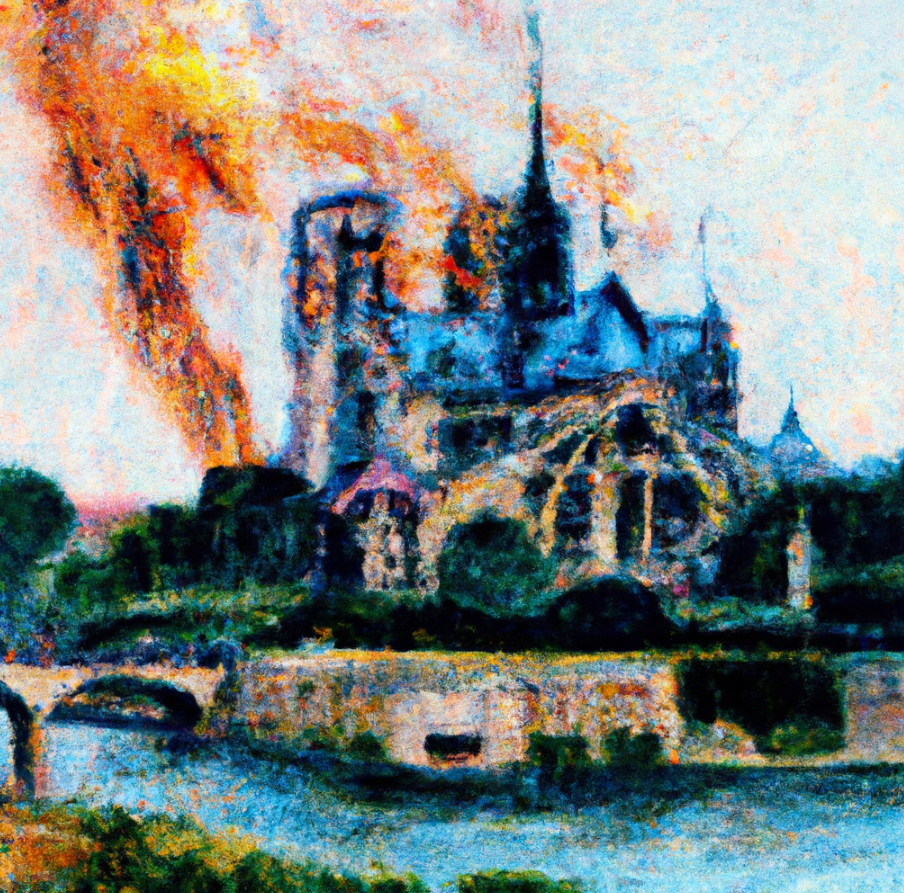
\includegraphics{./graphics/sample_5.png}} \\
        \hline
        \textbf{Referentie} &  \textbf{Sample 4} & \textbf{Sample 5} \\
        \hline
        Gebeurtenis &Terroristische aanslagen op het World Trade Center (11-9-2001) &  Brand in de Notre-Dame-kathedraal in Parijs.(15-4-2019) \\
        \hline
        Gebruikte prompt & 'Het verlies van onschuld en levens. Herdenk 9/11 met een modern kunstwerk in zwart-wit." - Stijl: Abstract-expressionisme.. & Symboliseer herstelkracht Notre-Dame na verwoestend vuur met hoopvolle, realistische elementen. Stijl: impressionisme. - Monet \\
        \hline
        Inspiratie (volgens GPT) & Mijn prompt was geen directe afspiegeling van een specifiek artikel of artikel titels. Het was bedoeld als een algemene prompt die de kernboodschap van de gebeurtenissen op 9/11 weergeeft in combinatie met de moderne kunststijl van het abstract-expressionisme in zwart-wit.& Ik heb me gebaseerd op de kernzin "Maak een kunstwerk dat de kracht en schoonheid van de Notre-Dame voorstelt, in combinatie met het tragische vuur dat de wereld heeft geschokt en de kracht van de menselijke spirit om te herstellen en te herbouwen." uit de vorige vraag. Voor deze prompt heb ik deze kernzin in een korte, bondige omschrijving omgezet die de artistieke stijl aangeeft \\
        \hline
    \end{tabular}
    \caption{Belangrijke gebeurtenissen gebruikt binnen de turingtest.}
    \label{table:events_samples}
\end{table}
\pagebreak
\section{Resultaat}
\label{section:result}
Binnen deze sectie zullen we kort de resultaten van de turingtest bespreken. \\

Bij de eerste 3 samples waarbij we op de huidige dag het nieuws hebben gescrapet, merken we op dat verschillende persona de schilderijen anders interpreteren. Dit kan te maken hebben met individuele smaak, persoonlijke achtergrond of andere factoren die van invloed zijn op hoe iemand kunstwerken waarneemt. Wat interessant is, is dat we hebben vastgesteld dat het al dan niet bekijken van het nieuws geen significante rol speelt bij de interpretatie van het schilderij. Dit suggereert dat de kunstwerken op zichzelf staan en geen specifieke voorkennis vereisen om begrepen te worden. \\

Daarnaast hebben we 2 samples gebruikt waarbij we gegevens hebben gescrapet van een specifieke dag in het verleden. Hierbij viel op dat de meeste personen de boodschap van deze kunstwerken konden afleiden. Dit duidt erop dat AI erin is geslaagd om de gewenste emotie of betekenis over te brengen op basis van belangrijke data uit het verleden.  \\

Hoewel er variatie was in de interpretaties van de kunstwerken, kunnen we concluderen dat de turingtest over het algemeen geslaagd is. Het vermogen van de kunstwerken om emoties op te roepen, betekenissen over te brengen en reacties uit te lokken, toont aan dat ze een waardevolle artistieke waarde hebben. Bovendien benadrukt het resultaat van de turingtest de veelzijdigheid en subjectiviteit van kunst. \\

De gedetailleerde resultaten van de turingtest zijn beschikbaar in bijlage punt \ref{bijlage:result_turingtest}. Daar kun je meer informatie vinden over de individuele interpretaties en feedback van de deelnemers.

 
\section{Meer uitleg}
Het resultaat verkregen van GPT en DALL-E is gebaseerd op patronen en informatie die het model heeft geleerd uit de gegevens waarop het is getraind. Hoewel deze modellen goede prestaties kunnen leveren, zijn er enkele beperkingen waardoor hun output niet altijd 100\% overeenkomt met de realiteit. \\

Ten eerste kan GPT soms de context of intentie van de invoer verkeerd begrijpen of verkeerd interpreteren. Dit kan leiden tot onjuiste of ongepaste antwoorden. Het model kan gevoelig zijn voor subtiele veranderingen in de formulering van de vraag en kan daardoor onverwachte resultaten produceren. \\

Ten tweede kan DALL-E, als een generatief model voor beeldcreatie, soms afbeeldingen genereren die niet volledig relevant zijn voor het huidige nieuws of specifieke vereisten. Hoewel het model in staat is om nieuwe, unieke afbeeldingen te maken op basis van de gegeven prompt, is het niet altijd in staat om contextuele nuances of specifieke details van de gewenste afbeelding te begrijpen. \\

We kunnen besluiten uit de werking van de applicatie dat doordat er nooit eenzelfde uitkomst is en deze uitkomst kan variëren in relevantie tot het nieuws, dat er steeds menselijke controle moet zijn op de foto vooraleer deze kan gebruikt worden binnen bijvoorbeeld een krant die dagelijks een kunstwerk genereert op basis van de artikels die hierin voorkomen. 
